\section{Teoria zstępowania i stosy}\label{cat:sec:descent-stacks}

Warunek snopu z rozdziału~\ref{cat:sec:grothendieck-topologies} pozwala sklejać lokalne sekcje, które są równe na przecięciach. Gdy lokalne dane są obiektami kategorii, np. przestrzeniami wektorowymi, wiązkami lub modułami, zamiast równości obiektów na przecięciach naturalnie pojawiają się izomorfizmy. Izomorfizmy te muszą spełniać warunek zgodności na potrójnych przecięciach. Teoria zstępowania (ang. \emph{descent theory}) bada, kiedy takie dane pochodzą od jednego obiektu globalnego i w jakim sensie obiekt ten jest jednoznaczny.

Korzystamy z języka fibracji Grothendiecka i pseudofunktorów z rozdziału~\ref{cat:sec:cartesian-fibrations}. Najpierw przedstawimy konstrukcję dla ścisłych funktorów kontrawariantnych; następnie uwzględnimy izomorfizmy koherencji i warunek stosu na miejscu Grothendiecka.

\subsection{Dane zstępowania dla rodziny morfizmów}

Niech $\mathcal B$ będzie kategorią mającą skończone iloczyny włókniste i niech $F:\mathcal B^{\mathrm{op}}\to\cat{Cat}$ będzie funktorem. Dla $f:V\to U$ piszemy $f^*=F(f):F(U)\to F(V)$. W tym podrozdziale mamy ścisłe równości $\id_U^*=\id_{F(U)}$ i $(fg)^*=g^*f^*$; nie zakładamy ich dla ogólnych pseudofunktorów.

Ustalmy rodzinę $\mathcal U=(u_i:U_i\to U)_{i\in I}$ indeksowaną zbiorem $I$. Kładziemy $U_{ij}=U_i\times_U U_j$ oraz $U_{ijk}=U_i\times_U U_j\times_U U_k$, z wybranymi iloczynami włóknistymi i ich rzutami. Symbole $\pi_1,\pi_2$ oznaczają rzuty z $U_{ij}$ na odpowiednio pierwszy i drugi czynnik, rozróżniając pozycje nawet wtedy, gdy $i=j$. Na $U_{ijk}$ symbole $\pi_{12},\pi_{23},\pi_{13}$ oznaczają rzuty do odpowiednich podwójnych iloczynów, a $\pi_1,\pi_2,\pi_3$ rzuty do pojedynczych czynników. Równości między złożeniami tych rzutów wynikają z ich własności uniwersalnych.

\begin{definicja}[Dane zstępowania]\label{cat:def:descent-datum}
Danymi zstępowania dla $F$ względem rodziny $\mathcal U$ nazywamy rodzinę obiektów $x_i\in F(U_i)$ oraz izomorfizmów
\[
 \theta_{ij}:\pi_2^*x_j\longrightarrow\pi_1^*x_i
 \qquad\text{w } F(U_{ij}),
\]
spełniających warunek diagonalny $\delta_i^*\theta_{ii}=\id_{x_i}$, gdzie $\delta_i:U_i\to U_{ii}$ jest diagonalą, oraz warunek kocyklu
\[
 \pi_{12}^*\theta_{ij}\circ\pi_{23}^*\theta_{jk}
 =\pi_{13}^*\theta_{ik}\qquad\text{w }F(U_{ijk}).
\]
Morfizm między danymi $(x_i,\theta_{ij})$ i $(y_i,\psi_{ij})$ jest rodziną $h_i:x_i\to y_i$, dla której
\[
 \psi_{ij}\circ\pi_2^*h_j=\pi_1^*h_i\circ\theta_{ij}
 \qquad\text{w }F(U_{ij}).
\]
\end{definicja}

Warunek kocyklu jest dobrze określony: po użyciu równości złożeń rzutów mamy diagram w $F(U_{ijk})$
\begin{center}
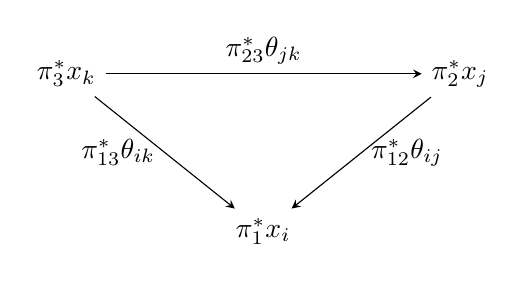
\begin{tikzpicture}[>=stealth]
 \node (z) at (0,0) {$\pi_3^*x_k$};
 \node (y) at (5,0) {$\pi_2^*x_j$};
 \node (x) at (2.5,-2) {$\pi_1^*x_i$};
 \draw[->] (z)--node[above] {$\pi_{23}^*\theta_{jk}$}(y);
 \draw[->] (y)--node[right] {$\pi_{12}^*\theta_{ij}$}(x);
 \draw[->] (z)--node[left] {$\pi_{13}^*\theta_{ik}$}(x);
\end{tikzpicture}
\end{center}
Wymagamy jego przemienności. Dla przejścia z $U_{ij}$ do $U_{ji}$ oznaczmy przez $s_{ij}$ izomorfizm zamieniający czynniki.

\begin{stwierdzenie}[Odwrócenie izomorfizmu przejścia]\label{cat:prop:descent-inverse}
Z warunków diagonalnego i kocyklu wynika
\[
 s_{ij}^*\theta_{ji}=\theta_{ij}^{-1}.
\]
\end{stwierdzenie}
\begin{proof}
Niech $a:U_{ij}\to U_{iji}$ będzie morfizmem o składowych $(\pi_1,\pi_2,\pi_1)$. Istnieje i jest jednoznaczny przez własność uniwersalną iloczynu włóknistego, gdyż wszystkie składowe mają to samo złożenie do $U$. Mamy $\pi_{12}a=\id_{U_{ij}}$, $\pi_{23}a=s_{ij}$ i $\pi_{13}a=\delta_i\pi_1$. Stosując $a^*$ do warunku kocyklu dla $(i,j,i)$, otrzymujemy
\[
 \theta_{ij}\circ s_{ij}^*\theta_{ji}
 =\pi_1^*\delta_i^*\theta_{ii}
 =\id_{\pi_1^*x_i}.
\]
Ponieważ $\theta_{ij}$ jest izomorfizmem, złożenie z jego odwrotnością daje tezę.
\end{proof}

Dane zstępowania wraz z powyższymi morfizmami tworzą kategorię, którą oznaczamy $\operatorname{Desc}_F(\mathcal U)$. Identyczności spełniają warunek morfizmu. Dla dwóch kolejnych morfizmów $h:(x,\theta)\to(y,\psi)$ i $g:(y,\psi)\to(z,\omega)$ mamy
\[
 \omega_{ij}\pi_2^*(g_jh_j)
 =\pi_1^*g_i\,\psi_{ij}\pi_2^*h_j
 =\pi_1^*(g_ih_i)\theta_{ij},
\]
więc złożenie składowe jest morfizmem danych zstępowania. Aksjomaty kategorii wynikają z aksjomatów w kategoriach $F(U_i)$.

\begin{stwierdzenie}[Funktor porównawczy]\label{cat:prop:descent-comparison}
Istnieje funktor
\[
 D_{\mathcal U}:F(U)\longrightarrow\operatorname{Desc}_F(\mathcal U),
\]
przypisujący obiektowi $x$ rodzinę $(u_i^*x)_i$ z identycznościowymi izomorfizmami przejścia, a morfizmowi $h$ rodzinę $(u_i^*h)_i$.
\end{stwierdzenie}
\begin{proof}
Równość $u_i\pi_1=u_j\pi_2$ daje ścisłą równość $\pi_1^*u_i^*x=\pi_2^*u_j^*x$, więc wskazane identyczności są poprawnie określone. Warunki diagonalny i kocyklu stają się równaniami identyczności. Dla $h:x\to y$ mamy $\pi_1^*u_i^*h=\pi_2^*u_j^*h$, co daje warunek morfizmu danych zstępowania. Zachowywanie identyczności i składania wynika z funktorialności wszystkich $u_i^*$.
\end{proof}

\begin{definicja}[Zstępowanie i efektywne zstępowanie]\label{cat:def:effective-descent}
Rodzinę $\mathcal U$ nazywamy rodziną zstępowania dla $F$, gdy $D_{\mathcal U}$ jest pełny i wierny, a rodziną efektywnego zstępowania, gdy $D_{\mathcal U}$ jest równoważnością kategorii. Dane zstępowania nazywamy efektywnymi, gdy są izomorficzne z obrazem pewnego obiektu $F(U)$.
\end{definicja}

Pełność i wierność wyrażają jednoznaczne sklejanie morfizmów; istotna surjektywność wyraża możliwość sklejenia obiektów. Jeżeli $D_{\mathcal U}$ jest pełny i wierny, to dla dwóch obiektów globalnych $x,y$ oraz ustalonego izomorfizmu $\varphi:D_{\mathcal U}x\to D_{\mathcal U}y$ istnieje dokładnie jeden izomorfizm $h:x\to y$ indukujący $\varphi$. Istnienie i jednoznaczność morfizmu wynikają z pełności i wierności. Stosując pełność do $\varphi^{-1}$, otrzymujemy $g:y\to x$; wierność daje $gh=\id_x$ i $hg=\id_y$. Nie twierdzimy, że $x,y$ są dosłownie tym samym obiektem.

\subsection{Związek z warunkiem snopu}

Dla zbioru $S$ oznaczamy przez $\operatorname{Disc}(S)$ kategorię dyskretną, której obiektami są elementy $S$, a jedynymi morfizmami są identyczności.

\begin{stwierdzenie}[Snop jako przypadek dyskretny]\label{cat:prop:descent-discrete-sheaf}
Niech $H:\mathcal B^{\mathrm{op}}\to\Set$ będzie presnopem i $F=\operatorname{Disc}\circ H$. Wówczas $D_{\mathcal U}$ jest równoważnością dokładnie wtedy, gdy funkcja
\[
 H(U)\longrightarrow
 \left\{(x_i)_i\in\prod_i H(U_i):
            \pi_1^*x_i=\pi_2^*x_j\text{ dla wszystkich }i,j\right\},
 \qquad x\longmapsto(u_i^*x)_i
\]
jest bijekcją.
\end{stwierdzenie}
\begin{proof}
W kategorii dyskretnej izomorfizm między dwoma obiektami istnieje dokładnie wtedy, gdy są one równe, i jest wówczas jedyny. Dlatego izomorfizmy $\theta_{ij}$ istnieją dokładnie dla rodzin spełniających wskazane równania; warunki diagonalny i kocyklu są wtedy automatyczne. Podobnie morfizm danych zstępowania istnieje tylko pomiędzy równymi rodzinami i jest identycznością. Kategoria danych zstępowania jest zatem dyskretną kategorią zgodnych rodzin. Funktor między kategoriami dyskretnymi jest pełny i wierny dokładnie wtedy, gdy funkcja na obiektach jest injekcją, oraz istotnie surjektywny dokładnie wtedy, gdy jest surjekcją. Zastosowanie tych kryteriów do $D_{\mathcal U}$ daje tezę.
\end{proof}

Jeżeli rodzina $\mathcal U$ generuje sito pokrywające $S$ na $U$, zgodne rodziny w powyższym wzorze odpowiadają naturalnym transformacjom $S\to H$. Istotnie, dla morfizmu $f:V\to U$ w $S$ wybieramy faktoryzację $f=u_i g$ i przypisujemy mu $g^*x_i$. Jeśli również $f=u_jh$, to istnieje morfizm $(g,h):V\to U_{ij}$; zastosowanie jego transportu do równania zgodności daje $g^*x_i=h^*x_j$. Przypisanie jest niezależne od faktoryzacji i naturalne względem prekompozycji, ponieważ $H$ jest funktorem. Odwrotnie, naturalna transformacja przypisuje $u_i$ element $x_i$; jej naturalność dla obu rzutów z $U_{ij}$ daje równanie zgodności. Obie konstrukcje są wzajemnie odwrotne. Jest to dokładnie warunek snopu z definicji~\ref{cat:def:site-sheaf}.

\subsection{Efektywne zstępowanie zbiorów wzdłuż surjekcji}

Rozważmy funkcję $u:V\to U$ i kategorię $\Set/U$ obiektów nad $U$. Jej obiekt $A\to U$ ma włókna $A_t$ dla $t\in U$, a morfizmy są funkcjami zachowującymi włókna. Równoważnie korzystamy z kategorii rodzin zbiorów $\Set^U$, gdzie $U$ jest kategorią dyskretną. Funktor $F$ przypisuje zbiorowi $U$ kategorię $\Set^U$, a funkcji $u:V\to U$ funktor prekompozycji, czyli $(u^*A)_v=A_{u(v)}$. W tym modelu transporty są ścisłe. Identyfikację z kategorią przekrojową otrzymujemy przez sumę rozłączną rodziny i przez branie włókien; obie konstrukcje są wzajemnie odwrotne z dokładnością do naturalnych izomorfizmów.

Dane zstępowania dla rodziny złożonej z $u$ to zbiory $A_v$ oraz bijekcje
\[
 \theta_{vw}:A_w\longrightarrow A_v
 \qquad(u(v)=u(w)),
\]
takie że $\theta_{vv}=\id$ i $\theta_{vw}\theta_{wz}=\theta_{vz}$, gdy $u(v)=u(w)=u(z)$.

\begin{twierdzenie}[Efektywne zstępowanie zbiorów]\label{cat:thm:set-effective-descent}
Dla funkcji $u:V\to U$ funktor porównawczy dla powyższego funktora $F$ jest równoważnością kategorii wtedy i tylko wtedy, gdy $u$ jest surjekcją.
\end{twierdzenie}
\begin{proof}
Załóżmy, że $u$ jest surjekcją. Dla danych zstępowania tworzymy zbiór $E=\coprod_{v\in V}A_v$, którego elementy zapisujemy jako $(v,a)$, $a\in A_v$. Definiujemy relację
\[
 (v,a)\sim(w,b)\quad\Longleftrightarrow\quad
 u(v)=u(w)\ \text{ i }\ a=\theta_{vw}(b).
\]
Relacja jest zwrotna przez warunek diagonalny. Jeżeli $(v,a)\sim(w,b)$, to $b=\theta_{wv}(a)$, ponieważ warunek kocyklu daje $\theta_{wv}\theta_{vw}=\theta_{ww}=\id$. Jeżeli ponadto $(w,b)\sim(z,c)$, to $a=\theta_{vw}\theta_{wz}(c)=\theta_{vz}(c)$ i wszystkie trzy elementy mają ten sam obraz w $U$. Otrzymujemy symetrię i przechodniość.

Niech $B=E/{\sim}$ z funkcją $B\to U$ daną przez $[(v,a)]\mapsto u(v)$, dobrze określoną z definicji relacji. Dla $v\in V$ definiujemy
\[
 \beta_v:A_v\longrightarrow B_{u(v)},\qquad
 a\longmapsto[(v,a)].
\]
Funkcja jest injektywna, ponieważ $[(v,a)]=[(v,b)]$ implikuje $a=\theta_{vv}(b)=b$. Jest też surjektywna: jeżeli $[(w,b)]\in B_{u(v)}$, to $u(w)=u(v)$ i $[(w,b)]=[(v,\theta_{vw}(b))]$. Wreszcie $\beta_v\theta_{vw}=\beta_w$, więc rodzina $\beta_v$ jest morfizmem danych zstępowania do $D_u(B)$. Każda składowa jest bijekcją, a składowe odwrotne również spełniają warunek morfizmu (otrzymujemy go przez złożenie równania zgodności z odwrotnościami). Stąd istotna surjektywność $D_u$.

Aby wykazać pełność i wierność, niech $B,C$ będą rodzinami na $U$. Morfizm $D_u(B)\to D_u(C)$ jest rodziną funkcji $h_v:B_{u(v)}\to C_{u(v)}$ spełniających $h_v=h_w$ dla $u(v)=u(w)$. Dla każdego $t\in U$ istnieje $v$ z $u(v)=t$. Definiujemy $h_t$ jako jedyną funkcję występującą w niepustej rodzinie $\{h_v:u(v)=t\}$; jej jednoznaczność wynika z warunku zgodności. Otrzymana rodzina $h=(h_t)_t$ jest morfizmem $B\to C$, którego obraz to rodzina $(h_v)_v$. Każda inna rodzina o tym obrazie ma te same składowe, ponieważ $u$ jest surjektywna. To daje pełność i wierność.

Odwrotnie, jeśli $u$ nie jest surjekcją, wybierzmy $t_0\in U\setminus u(V)$. Niech $B_t=\{*\}$ dla wszystkich $t$, $C_{t_0}=\{0,1\}$, a $C_t=\{*\}$ dla pozostałych $t$. Istnieją dwa różne morfizmy $B\to C$, różniące się wartością w składowej $t_0$. Ich obrazy przez $D_u$ są równe, bo żadna składowa nad $V$ nie widzi $t_0$. Funktor $D_u$ nie jest wierny, a zatem nie jest równoważnością.
\end{proof}

\begin{przyklad}[Sklejenie dwóch kopii zbioru]\label{cat:ex:set-descent-two-copies}
Niech $U=\{*\}$, $V=\{1,2\}$, a $u$ będzie jedyną funkcją. Dane zstępowania składają się z dwóch zbiorów $A_1,A_2$ i bijekcji $\theta:A_2\to A_1$; pozostałe izomorfizmy to identyczności i $\theta^{-1}$. Iloraz z dowodu twierdzenia~\ref{cat:thm:set-effective-descent} utożsamia $(2,b)$ z $(1,\theta(b))$. Zbiór globalny jest więc kanonicznie izomorficzny z $A_1$ (i z $A_2$ za pomocą $\theta$). Nawet gdy $A_1,A_2$ są rozłącznymi zbiorami, dane mogą być efektywne: wymagana jest zgodność przez izomorfizm, a nie równość lokalnych obiektów.
\end{przyklad}

\subsection{Zstępowanie w fibracji Grothendiecka}

Niech $p:\mathcal E\to\mathcal B$ będzie fibracją Grothendiecka. Włókno nad $U$ oznaczamy przez $\mathcal E_U$. Wybieramy podniesienia kartezjańskie $\lambda_{f,x}:f^*x\to x$ nad $f:V\to U$ jak w definicji~\ref{cat:def:grothendieck-fibration}. Porównania transportów $c_{f,g}:f^*g^*\Rightarrow(gf)^*$ i $e_U:\id\Rightarrow(\id_U)^*$ są określone przez twierdzenie~\ref{cat:thm:reindexing-pseudofunctor}. Poniższa konstrukcja nie wymaga rozszczepienia fibracji.

Dla rodziny $\mathcal U=(u_i:U_i\to U)_i$ używamy iloczynów włóknistych i oznaczeń z definicji~\ref{cat:def:descent-datum}. Niech $v_{ij}:U_{ij}\to U$ oznacza wspólne złożenie $u_i\pi_1=u_j\pi_2$.

\begin{definicja}[Dane zstępowania w fibracji]\label{cat:def:fibered-descent}
Dane zstępowania składają się z obiektów $x_i\in\mathcal E_{U_i}$ oraz pionowych izomorfizmów
\[
 \theta_{ij}:\pi_2^*x_j\longrightarrow\pi_1^*x_i.
\]
Dla $a:V\to U_{ij}$ definiujemy izomorfizm
\[
 \theta_{ij}[a]=c_{a,\pi_1,x_i}\,a^*(\theta_{ij})\,
                         c_{a,\pi_2,x_j}^{-1}
 :(\pi_2a)^*x_j\longrightarrow(\pi_1a)^*x_i.
\]
Warunek diagonalny ma postać $\theta_{ii}[\delta_i]=\id_{(\id_{U_i})^*x_i}$, a warunek kocyklu
\[
 \theta_{ij}[\pi_{12}]\theta_{jk}[\pi_{23}]
 =\theta_{ik}[\pi_{13}].
\]
Morfizmy są rodzinami pionowych morfizmów $h_i:x_i\to y_i$, spełniającymi $\psi_{ij}\pi_2^*h_j=\pi_1^*h_i\theta_{ij}$.
\end{definicja}

Warunek diagonalny można równoważnie zapisać na obiekcie $x_i$ przez sprzężenie izomorfizmem $e_{U_i,x_i}$. Jeżeli transporty są ścisłe i porównania identycznościowe, otrzymujemy definicję~\ref{cat:def:descent-datum}. Morfizmy składają się składowo: dowód jest taki sam jak w przypadku ścisłym, ponieważ każdy pojedynczy transport jest zwykłym funktorem.

\begin{stwierdzenie}[Porównanie po dalszej zmianie bazy]\label{cat:prop:descent-transport-coherence}
Niech $\vartheta:f^*x\to g^*y$ będzie morfizmem w $\mathcal E_V$, gdzie $f:V\to U$, $g:V\to W$, $x\in\mathcal E_U$, $y\in\mathcal E_W$. Dla $a:T\to V$ i $b:S\to T$ kładziemy
\[
 \vartheta[a]=c_{a,g,y}\,a^*(\vartheta)\,c_{a,f,x}^{-1}.
\]
Wówczas $\vartheta[a][b]=\vartheta[ab]$, przy czym po pierwszym transporcie stosujemy definicję do morfizmów $fa$ i $ga$. Ponadto transport zachowuje identyczności i składanie odpowiednio typowanych morfizmów.
\end{stwierdzenie}
\begin{proof}
Rozwijając dwukrotny transport, dostajemy
\[
 c_{b,ga,y}\,b^*(c_{a,g,y})\,b^*a^*(\vartheta)\,
 b^*(c_{a,f,x}^{-1})\,c_{b,fa,x}^{-1}.
\]
Z równania koherencji~\eqref{cat:eq:transport-associativity} dwa lewe czynniki są równe $c_{ab,g,y}c_{b,a,g^*y}$. Dwa prawe czynniki są odwrotnością $c_{b,fa,x}b^*(c_{a,f,x})$, a zatem są równe $c_{b,a,f^*x}^{-1}c_{ab,f,x}^{-1}$. Naturalność $c_{b,a}$ daje
\[
 c_{b,a,g^*y}\,b^*a^*(\vartheta)\,c_{b,a,f^*x}^{-1}
 =(ab)^*(\vartheta).
\]
Po podstawieniu otrzymujemy $\vartheta[ab]$. Przy składaniu dwóch morfizmów środkowe czynniki porównawcze skracają się wzajemnie, a $a^*$ zachowuje składanie. Dla identyczności porównanie i jego odwrotność również się skracają.
\end{proof}

\begin{stwierdzenie}[Globalne dane zstępowania w fibracji]\label{cat:prop:fibered-descent-comparison}
Dla $x\in\mathcal E_U$ rodzina $x_i=u_i^*x$ z izomorfizmami
\[
 \theta_{ij}=c_{\pi_1,u_i,x}^{-1}c_{\pi_2,u_j,x}
\]
jest danymi zstępowania. Przypisanie tych danych do $x$ oraz rodziny $(u_i^*h)_i$ do pionowego morfizmu $h$ określa funktor porównawczy.
\end{stwierdzenie}
\begin{proof}
Oba porównania w definicji $\theta_{ij}$ mają przeciwdziedzinę $v_{ij}^*x$, więc złożenie jest dobrze określone. Dla $a:T\to U_{ij}$ z równania koherencji otrzymujemy
\[
 \theta_{ij}[a]=c_{\pi_1a,u_i,x}^{-1}c_{\pi_2a,u_j,x}.
\]
Istotnie, rozwijamy definicję transportu $\theta_{ij}[a]$ i stosujemy koherencję do trójek $a,\pi_1,u_i$ oraz $a,\pi_2,u_j$; wspólny czynnik $c_{a,v_{ij},x}$ skraca się. Dla $a=\delta_i$ oba porównania są takie same, co daje warunek diagonalny. Na $U_{ijk}$ mamy zatem
\[
 \theta_{ij}[\pi_{12}]\theta_{jk}[\pi_{23}]
 =(c_{\pi_1,u_i,x}^{-1}c_{\pi_2,u_j,x})
   (c_{\pi_2,u_j,x}^{-1}c_{\pi_3,u_k,x})
 =\theta_{ik}[\pi_{13}].
\]
Naturalność porównań względem $h:x\to y$ daje zgodność morfizmów lokalnych z przejściami. Funktorialność wynika z funktorialności transportów.
\end{proof}

\subsection{Opis niezależny od wyboru podniesień}

Dla sita $R$ na $U$ traktujemy $R$ jako pełną podkategorię $\mathcal B/U$ złożoną z morfizmów należących do sita. Funktor dziedziny $d_R:R\to\mathcal B$ wysyła $f:V\to U$ na $V$, a morfizm $a:f\to g$ na funkcję bazową $a$ spełniającą $ga=f$ (w ogólnej kategorii jest to morfizm, niekoniecznie funkcja).

\begin{definicja}[Kartezjańska sekcja nad sitem]\label{cat:def:descent-sieve-section}
Przez $\operatorname{Cart}(R,\mathcal E)$ oznaczamy kategorię funktorów $s:R\to\mathcal E$, takich że $ps=d_R$ i każdy morfizm $s(a)$ jest kartezjański. Morfizmy są transformacjami naturalnymi $\alpha:s\Rightarrow t$ o pionowych składowych, czyli $p(\alpha_f)=\id_{d_R(f)}$.
\end{definicja}

Jest to definicja niewykorzystująca żadnego wyboru podniesień. Dla obiektu $x\in\mathcal E_U$ wybrane podniesienia określają sekcję $s_x(f)=f^*x$, gdzie dla $a:f\to g$ morfizm $s_x(a)$ jest jedynym morfizmem nad $a$ spełniającym $\lambda_{g,x}s_x(a)=\lambda_{f,x}$. Istnienie i jednoznaczność daje kartezjańskość $\lambda_{g,x}$; kartezjańskość $s_x(a)$ wynika ze stwierdzenia~\ref{cat:prop:cartesian-composition}. Identyczności i składanie zachodzą przez jednoznaczność po złożeniu z odpowiednim $\lambda$. Pionowy morfizm $h:x\to y$ daje naturalną transformację o składowych $f^*h$: obie strony równania naturalności mają po złożeniu z $\lambda_{g,y}$ wartość $h\lambda_{f,x}$. Otrzymujemy funktor $D_R:\mathcal E_U\to\operatorname{Cart}(R,\mathcal E)$. Dwa wybory podniesień dają naturalnie izomorficzne funktory: jedyne pionowe izomorfizmy między podniesieniami są naturalne względem morfizmów sita i względem $x$, ponownie przez jednoznaczność faktoryzacji.

\begin{stwierdzenie}[Sito maksymalne]\label{cat:prop:descent-maximal-sieve}
Dla sita maksymalnego $h_U=\mathcal B/U$ funktor $D_{h_U}$ jest równoważnością kategorii.
\end{stwierdzenie}
\begin{proof}
Funktor ewaluacji $\operatorname{ev}_{\id_U}$ przypisuje sekcji $s$ obiekt $s(\id_U)$ i transformacji jej składową w $\id_U$. Złożenie $\operatorname{ev}_{\id_U}D_{h_U}$ jest naturalnie izomorficzne z identycznością przez porównanie jednostkowe $e_U$. Dla dowolnej sekcji $s$ i $f:V\to U$ istnieje jedyny morfizm $f\to\id_U$ w kategorii przekrojowej, o składowej bazowej $f$. Jego obraz $s(f)\to s(\id_U)$ jest kartezjański. Porównując go z wybranym podniesieniem $\lambda_{f,s(\id_U)}$, otrzymujemy jedyny pionowy izomorfizm $s(f)\to f^*s(\id_U)$. Izomorfizmy te są naturalne względem $f$: dla morfizmu $a:f\to g$ obie strony równania naturalności po złożeniu z $\lambda_{g,s(\id_U)}$ są obrazem jedynego morfizmu $f\to\id_U$. Są również naturalne względem transformacji sekcji, ponieważ jej naturalność dla morfizmu $f\to\id_U$ daje wymaganą równość po złożeniu z podniesieniem. Otrzymujemy naturalny izomorfizm $\id\Rightarrow D_{h_U}\operatorname{ev}_{\id_U}$, co kończy dowód.
\end{proof}

\begin{twierdzenie}[Porównanie opisu przez rodzinę i przez sito]\label{cat:thm:descent-family-sieve}
Jeżeli $\mathcal B$ ma iloczyny włókniste, a $R$ jest sitem generowanym przez rodzinę $\mathcal U=(u_i)_i$, to kategoria $\operatorname{Cart}(R,\mathcal E)$ jest równoważna kategorii danych zstępowania z definicji~\ref{cat:def:fibered-descent}. Równoważność identyfikuje funktory porównawcze z dokładnością do naturalnego izomorfizmu.
\end{twierdzenie}
\begin{proof}
Dla sekcji $s$ bierzemy $x_i=s(u_i)$. Na $U_{ij}$ obiekt $s(v_{ij})$ ma kartezjańskie morfizmy do $x_i,x_j$ nad $\pi_1,\pi_2$, otrzymane z morfizmów w sicie. Porównanie z wybranymi podniesieniami daje pionowe izomorfizmy
\[
 l_{ij,1}:s(v_{ij})\longrightarrow\pi_1^*x_i,\qquad
 l_{ij,2}:s(v_{ij})\longrightarrow\pi_2^*x_j.
\]
Definiujemy $\theta_{ij}=l_{ij,1}l_{ij,2}^{-1}$. Na potrójnym iloczynie włóknistym porównujemy wspólny obiekt sekcji z trzema transportami $\pi_1^*x_i,\pi_2^*x_j,\pi_3^*x_k$. Oznaczmy otrzymane izomorfizmy przez $L_1,L_2,L_3$. Z jednoznaczności kartezjańskiej faktoryzacji i równania~\eqref{cat:eq:transport-comparison} wynika $\theta_{ij}[\pi_{12}]=L_1L_2^{-1}$: obie składowe porównania są uzyskane przez złożenie podniesień nad odpowiednimi rzutami. Analogicznie dostajemy $L_2L_3^{-1}$ i $L_1L_3^{-1}$ dla pozostałych par, więc kocykl zachodzi. Na przekątnej obie porównywane strzałki sekcji są tym samym morfizmem, co daje warunek diagonalny. Naturalna transformacja sekcji daje rodzinę $h_i$ spełniającą zgodność z $\theta_{ij}$ przez naturalność dla obu rzutów. Tak otrzymujemy funktor $K$.

Dla danych zstępowania $(x_i,\theta_{ij})$ wybieramy dla każdego $f:V\to U$ w $R$ jedną faktoryzację $f=u_{i(f)}b_f$. Kładziemy $s(f)=b_f^*x_{i(f)}$. Aby opisać morfizmy i sprawdzić funktorialność, dla dowolnych dwóch faktoryzacji $f=u_i b=u_j c$ definiujemy
\[
 T_{b,c}=\theta_{ij}[(b,c)]:c^*x_j\longrightarrow b^*x_i,
\]
gdzie $(b,c):V\to U_{ij}$ jest wyznaczony przez własność uniwersalną. Warunek kocyklu, zastosowany po transporcie przez $(b,c,d):V\to U_{ijk}$ i stwierdzenie~\ref{cat:prop:descent-transport-coherence}, daje $T_{b,c}T_{c,d}=T_{b,d}$. Warunek diagonalny daje $T_{b,b}=\id$ przez faktoryzację $(b,b)=\delta_i b$ i to samo stwierdzenie. Dla $a:W\to V$ mamy dodatkowo
\[
 T_{ba,ca}=c_{a,b,x_i}\,a^*(T_{b,c})\,c_{a,c,x_j}^{-1}.
\]
Jest to bezpośrednio równanie o dalszej zmianie bazy.

Dla morfizmu $a:f\to g$ w $R$ (czyli $ga=f$) definiujemy
\[
 s(a)=\lambda_{b_g,x_{i(g)}}^{\,a}\,
       c_{a,b_g,x_{i(g)}}^{-1} T_{b_ga,b_f},
 \qquad
 \lambda_{b_g,x_{i(g)}}^{\,a}:=\lambda_{a,b_g^*x_{i(g)}}.
\]
Pierwsze dwa czynniki po $T$ mają dziedzinę $(b_ga)^*x_{i(g)}$ i przeciwdziedzinę $s(g)$, a ich złożenie jest kartezjańskie nad $a$. Ponieważ $T$ jest pionowym izomorfizmem, cały morfizm jest kartezjański.

Dla sprawdzenia składania niech $a:f\to g$ i $d:g\to h$. Wygodnie oznaczyć składową pionową $s(a)$ względem $\lambda_{a,s(g)}$ przez
\[
 A=c_{a,b_g}^{-1}T_{b_ga,b_f},\qquad
 B=c_{d,b_h}^{-1}T_{b_hd,b_g}
\]
dla $s(d)$. Pomijamy indeks obiektu przy porównaniach, gdy wynika z typów. Składowa pionowa $s(d)s(a)$ względem podniesienia nad $da$ to $c_{a,d}a^*(B)A$, zgodnie z równaniem~\eqref{cat:eq:transport-comparison} i naturalnością podniesień. Stosując równanie dla $T$ po zmianie bazy, dostajemy
\[
\begin{aligned}
 c_{a,d}a^*(B)A
 &=c_{a,d}a^*(c_{d,b_h}^{-1})\,
   c_{a,b_hd}^{-1}T_{b_hda,b_ga}T_{b_ga,b_f}\\
 &=c_{da,b_h}^{-1}T_{b_hda,b_f}.
\end{aligned}
\]
W pierwszej równości skróciły się czynniki $c_{a,b_g}$ i jego odwrotność, w drugiej użyliśmy koherencji porównań oraz kocyklu dla $T$. To jest składowa pionowa $s(da)$. Dla $a=\id$ mamy $T_{b_f,b_f}=\id$ oraz $c_{\id,b_f}^{-1}=e_{V,b_f^*x_{i(f)}}$, więc z równania jednostki podniesień $s(\id)=\id$. Otrzymujemy sekcję.

Dla morfizmu danych $h_i:x_i\to y_i$ bierzemy na $f$ morfizm $b_f^*h_{i(f)}$. Zgodność z $\theta$ po transporcie daje zgodność z $T_{b,c}$, a naturalność porównań i podniesień daje naturalność względem $s(a)$. Konstrukcja zachowuje identyczności i składanie składowo, więc określa funktor $L$.

Dla danych $(x_i,\theta_{ij})$ porównujemy $K L(x_i,\theta_{ij})$ z danymi wyjściowymi. Na $u_i$ mamy faktoryzację wybraną $u_i=u_{i(u_i)}b_{u_i}$ oraz faktoryzację $u_i=u_i\id$. Izomorfizm do $x_i$ jest złożeniem $T_{\id,b_{u_i}}$ z $e_{U_i,x_i}^{-1}$. Zgodność z przejściami wynika z równania $T_{b,c}T_{c,d}=T_{b,d}$ i jego transportu: na $U_{ij}$ każda droga porównuje te same faktoryzacje $v_{ij}$, więc daje ten sam izomorfizm. Naturalność względem morfizmów danych wynika z ich zgodności z $T$.

Dla sekcji $s$ i $f=u_i b_f$ kartezjański morfizm $s(f)\to s(u_i)$ nad $b_f$ daje jedyny pionowy izomorfizm $s(f)\to b_f^*s(u_i)=LK(s)(f)$. Dla dwóch faktoryzacji $f=u_i b=u_j c$ porównania tego samego obiektu $s(f)$ z $b^*s(u_i)$ i $c^*s(u_j)$ różnią się przez $T_{b,c}$: jest to definicja $\theta_{ij}$ po transporcie przez $(b,c)$. Dlatego izomorfizmy $s(f)\to LK(s)(f)$ są naturalne względem morfizmów sita (po złożeniu z podniesieniem nad $a$ obie strony dają ten sam morfizm). Naturalność względem transformacji sekcji wynika z naturalności dla morfizmu $f\to u_i$. Otrzymujemy naturalne izomorfizmy $KL\cong\id$ i $\id\cong LK$. Dla sekcji pochodzącej od obiektu globalnego porównania na $U_{ij}$ są dokładnie porównaniami z twierdzenia~\ref{cat:prop:fibered-descent-comparison}, zatem $K D_R\cong D_{\mathcal U}$.
\end{proof}

\subsection{Prestosy i stosy na miejscu Grothendiecka}

Niech $(\mathcal B,J)$ będzie małym miejscem w sensie definicji~\ref{cat:def:grothendieck-topology}, a $p:\mathcal E\to\mathcal B$ fibracją o lokalnie małych włóknach; przy większych kategoriach ustalamy odpowiednie uniwersa.

\begin{definicja}[Prestos i stos]\label{cat:def:prestack-stack}
Fibrację $p$ nazywamy prestosem, jeżeli dla każdego $U\in\mathcal B$ i każdego sita pokrywającego $R\in J(U)$ funktor $D_R$ jest pełny i wierny. Nazywamy ją stosem, jeżeli dla wszystkich takich sit $D_R$ jest równoważnością kategorii. Stos w grupoidach to stos, którego wszystkie włókna są grupoidami.
\end{definicja}

Terminologia nie jest jednolita: niektórzy autorzy nazywają prestosem dowolną fibrację lub pseudofunktor, a dodatkowy warunek pełności i wierności nazywają rozdzielonością. Tutaj przyjmujemy definicję~\ref{cat:def:prestack-stack}. Twierdzenie~\ref{cat:thm:descent-family-sieve} pozwala sprawdzać warunki za pomocą rodzin pokrywających, gdy istnieją iloczyny włókniste. Na małym miejscu każde sito jest generowane przez rodzinę wszystkich swoich morfizmów.

Dla $x,y\in\mathcal E_U$ definiujemy presnop morfizmów na kategorii przekrojowej $\mathcal B/U$ przez
\[
 \mathcal H_{x,y}(f:V\to U)
 =\Hom_{\mathcal E_V}(f^*x,f^*y).
\]
Dla $a:f\to g$ transport jest dany wzorem
\[
 \mathcal H_{x,y}(a)(h)
 =c_{a,g,y}\,a^*(h)\,c_{a,g,x}^{-1}.
\]
Zgodność ze składaniem wynika ze stwierdzenia~\ref{cat:prop:descent-transport-coherence}; dla identyczności korzystamy z równania jednostki $c_{\id,g}=e^{-1}$ i naturalności $e$. Jest to więc presnop zbiorów.

Topologię na kategorii przekrojowej określamy następująco: sito na obiekcie $f:V\to U$ pokrywa, jeżeli odpowiadające mu sito morfizmów do $V$ należy do $J(V)$. Odpowiedniość sit wynika z faktu, że morfizm do $f$ w kategorii przekrojowej jest jednoznacznie wyznaczony przez morfizm $a:W\to V$ (jego dziedziną jest $fa$). Identyczność, zmiana bazy i lokalność pokrycia przenoszą się z $J$.

\begin{twierdzenie}[Kryterium prestosu przez snopy morfizmów]\label{cat:thm:prestack-hom-sheaf}
Fibracja $p$ jest prestosem wtedy i tylko wtedy, gdy dla każdego $U$ i każdych $x,y\in\mathcal E_U$ presnop $\mathcal H_{x,y}$ jest snopem na $\mathcal B/U$.
\end{twierdzenie}
\begin{proof}
Dla sita $R$ na $U$ morfizm $D_R(x)\to D_R(y)$ jest rodziną pionowych morfizmów $h_f:f^*x\to f^*y$, naturalną względem morfizmów $a:f\to g$ w $R$. Równanie naturalności jest równoważne
\[
 h_f=c_{a,g,y}\,a^*(h_g)\,c_{a,g,x}^{-1}.
\]
Istotnie, morfizm sekcji $s_x(a)$ to $\lambda_{a,g^*x}c_{a,g,x}^{-1}$, analogicznie dla $y$. Po podstawieniu do równania naturalności korzystamy z naturalności podniesienia i jego jednoznacznej faktoryzacji. Otrzymujemy dokładnie zgodną rodzinę sekcji presnopu $\mathcal H_{x,y}$ nad sitem na obiekcie $\id_U$ w $\mathcal B/U$. Sekcje nad $\id_U$ są kanonicznie identyfikowane z $\Hom_{\mathcal E_U}(x,y)$ przez porównanie $e_U$. Funkcja ograniczenia jest więc bijekcją wtedy i tylko wtedy, gdy $D_R$ indukuje bijekcję na tym zbiorze morfizmów.

Jeżeli wszystkie $\mathcal H_{x,y}$ są snopami, stosujemy ten warunek do $\id_U$ i wszystkich sit pokrywających, uzyskując pełność i wierność. Odwrotnie, załóżmy, że $p$ jest prestosem. Dla dowolnego $g:V\to U$ presnop $\mathcal H_{x,y}$ ograniczony do kategorii obiektów nad $g$ jest naturalnie izomorficzny z $\mathcal H_{g^*x,g^*y}$ na $\mathcal B/V$. Na morfizmie $a:W\to V$ izomorfizm jest dany przez $h\mapsto c_{a,g,y}^{-1}h c_{a,g,x}$. Jego naturalność wynika z równania koherencji dla dwóch kolejnych zmian bazy. Pełność i wierność $D_S$ dla każdego sita pokrywającego $S$ na $V$ dają z pierwszej części warunek snopu na $g$. Ponieważ $g$ było dowolne, presnop jest snopem na całej kategorii przekrojowej.
\end{proof}

\begin{wniosek}[Lokalne wykrywanie izomorfizmów]\label{cat:cor:prestack-local-isomorphisms}
Jeżeli $p$ jest prestosem, a pionowy morfizm $h:x\to y$ nad $U$ po każdym transporcie wzdłuż morfizmu sita pokrywającego $R$ staje się izomorfizmem, to $h$ jest izomorfizmem.
\end{wniosek}
\begin{proof}
Morfizm $D_R(h)$ jest izomorfizmem, ponieważ jego wszystkie składowe są izomorfizmami, a odwrotności składowe tworzą transformację naturalną. Pełność daje pionowy morfizm $g:y\to x$, którego obraz jest odwrotnością $D_R(h)$. Wierność daje $gh=\id_x$ i $hg=\id_y$.
\end{proof}
